\chapter{Arm Cortex-M4 Processor and Its
Architecture}

\section{What is an ARM architecture?}

ARM stands for \textbf{Advanced RISC Machine}. It's a family of RISC-based processors, well-known for their
power efficiency and use in mobile devices (smartphones and tablets), designed and licensed by Arm to a
wide ecosystem of partners.

\section{RISC VS CISC}


\paragraph{Complex Instruction Set Computer (CISC):}
\paragraph{}
This processor offers a variety of instructions that perform very complex tasks like string searching and a
number of different instruction formats of varying lengths.

Examples of CISC processors are Intel processors.

\paragraph{Reduced Instruction Set Computer (RISC):}
\paragraph{}

This processor offers fewer and simpler instructions that can be efficiently executed in a pipelined manner,generally uses load/store instruction sets, operates only on register and cannot operate directly on
memory locations.


Overall, it's simplified hardware design and implementation which means that it will require less
power to use.


What is an ARM Cortex processor? What does it offer us? What are they main components?


\section{ARM Company}

Arm is the company that designs Arm-based processor cores. It does not manufacture them, but licenses
the designs to semiconductor partners which can add their own intellectual property (IP) on top of, which
then can fabricate and sell to customers.


\paragraph{}
Two types of licenses:

\begin{itemize}
    \item Microarchitectural License, which allows the vendor to use one of the various available Cortex licenses (RTL-level design of the processor).
    \item Architectural License, which allows the vendor to develop one's own microarchitecture based on ARM's ISA.
\end{itemize}

\section{How to Design an Arm-based SoC}

\begin{enumerate}
    \item Select a set of IP cores from Arm and/or other third-party IP vendors
    \item Integrate IP cores into a single-chip design
    \item Give design to semiconductor foundries for chip fabrication
\end{enumerate}

\begin{figure}[H]
    \centering
    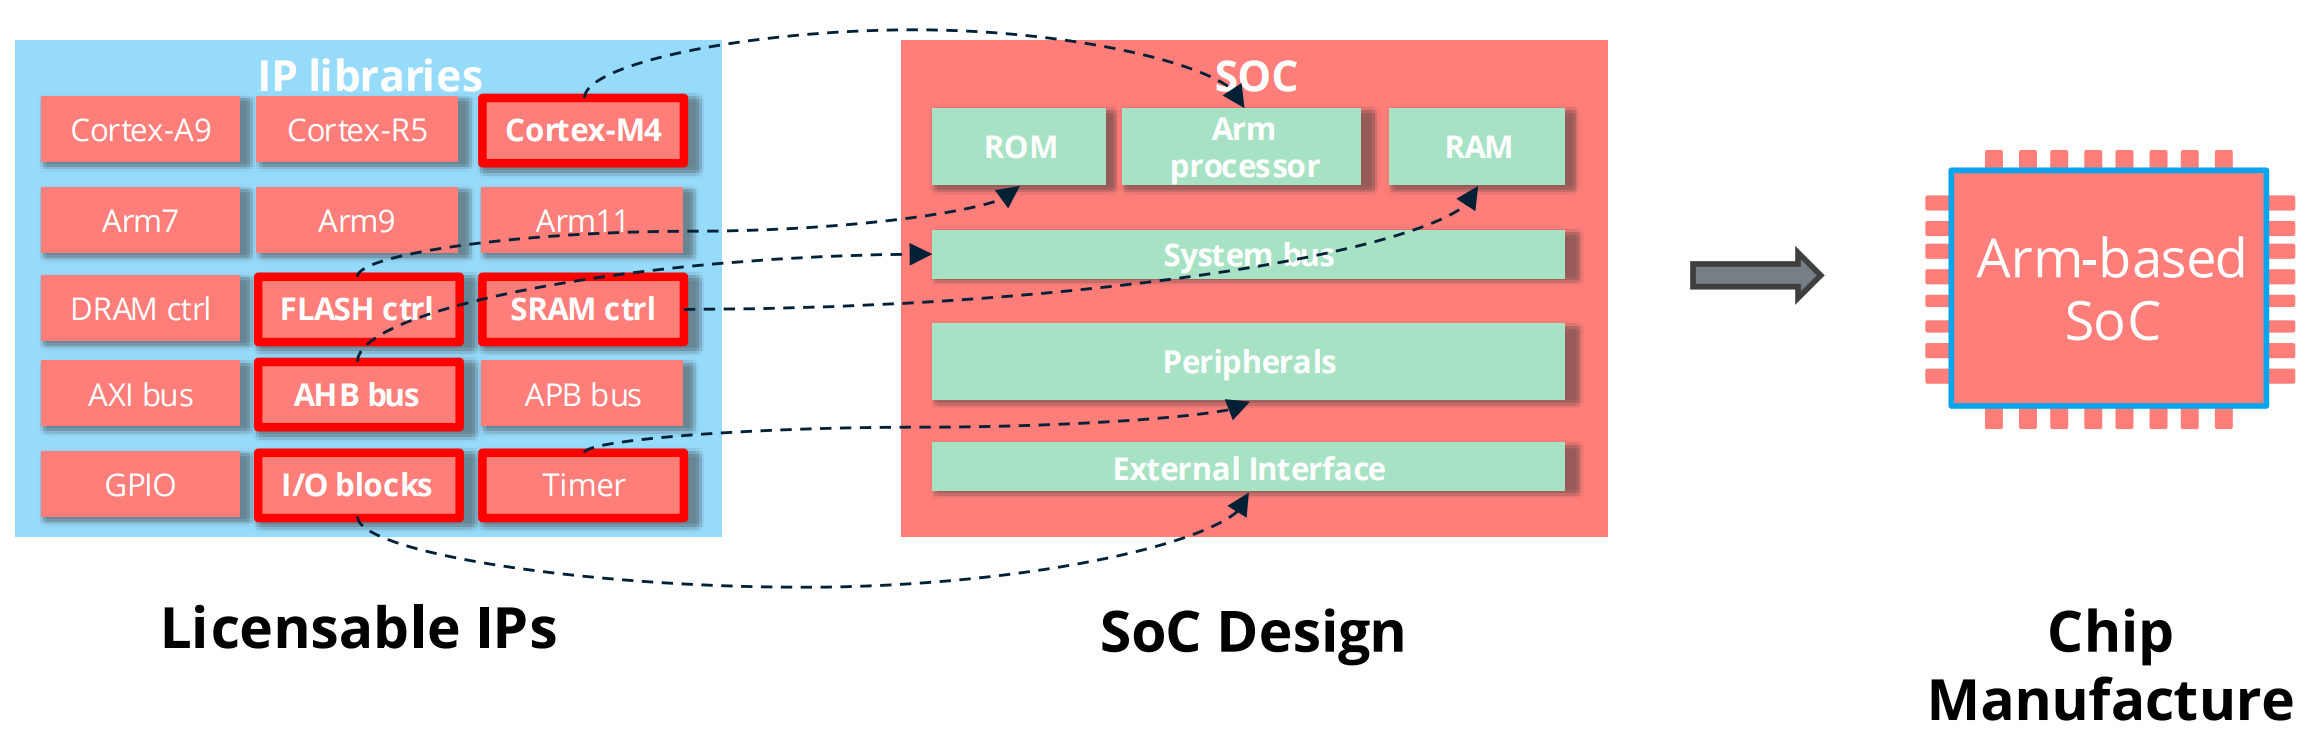
\includegraphics[width=1\linewidth]{img/image8.png}
\end{figure}

\section{Arm Processor Families}

\subsection*{Cortex-A series (Application)}
High performance processors capable of full operating system (OS) support. Applications include smartphones, digital TV, smart books.


\subsection*{Cortex-R series (Real-time)}
High performance and reliability for real-time applications. Applications include automotive braking systems, powertrains.


\subsection*{Cortex-M series (Microcontroller)}  

Cost sensitive solutions for deterministic microcontroller applications. Applications include microcontrollers, smart sensors.


\section{Arm Cortex-M Series}

The main features of a Cortex-M series processor are:

\begin{itemize}
    \item Energy efficiency
    \\ Low energy cost, which means longer battery life
    \item Smaller code
    \\ The code is smaller which means less memory is required, which means less power is consumed and hardware costs are lower
    \item Lower silicon costs
    \\ They occupy less physical space
    \item Ease of use and development
    \\ Faster software development and reuse (lots of tools)
    \item Targets several embedded applications
    \\ Like smart metering, human interface devices, automotive and industrial control systems, white goods (home appliances), consumer products and medical instrumentation
\end{itemize}

\section{Cortex-M series processors ranked}
The higher the number the better.

\subsection*{Cortex-M0 and Cortex M0+}

Cortex-M0 and Cortex-M0+ are for \textbf{applications requiring minimal cost, power and space}.
They're optimized for simple sensing and controlling.

\subsection*{Cortex-M3, Cortex-M4 and Cortex-M7}

These are \textbf{designed for data intensive applications requiring
higher performance}, like digital signal control applications. 

Cortex-M4 and Cortex-M7 integrate Digital Signal Processing (\textbf{DSP}) and \textbf{accelerated floating point processing capability} for fast and
power-efficient algorithm processing.

\section{Architectures and Implementations}

The architecture is the Instruction Set Architecture (ISA), which defines those characteristics and
instructions that must be true for all implementations.

Implementations are the actual hardware implementations of the architecture, which can have varying
clock speeds, different bus widths, different cache sizes and so on.


\section{Arm Architectures vs.Arm Processors}

\subsection*{Arm architecture}

The Arm architecture \textbf{describes the details of the instruction set}, the programmer's model, memory map.

\paragraph{}
Overtime, Arm architecture evolved to include architectural features that meet the growing demand for
new functionality (example: AI), integrated security features, high performance and the needs of new and
emerging markets.

\subsection*{Arm Processors}

The Arm processor is the implementation of the Arm architecture.

\begin{figure}[H]
    \centering
    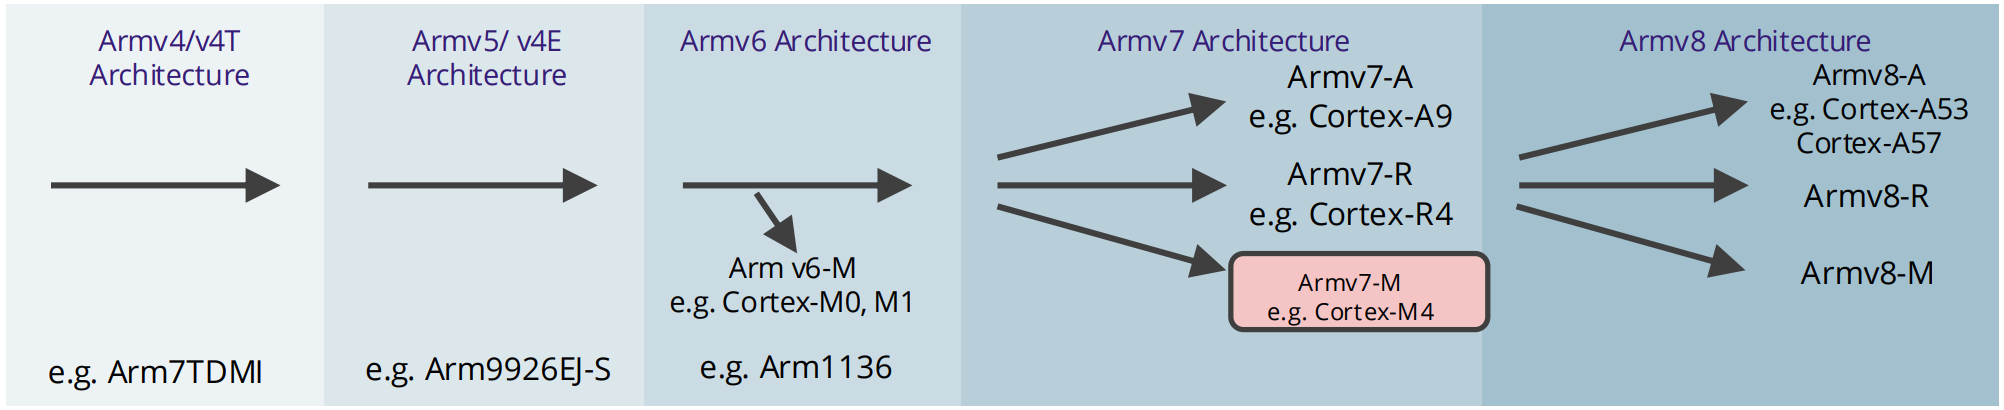
\includegraphics[width=1\linewidth]{img/image9.png}
\end{figure}

\begin{figure}[H]
    \centering
    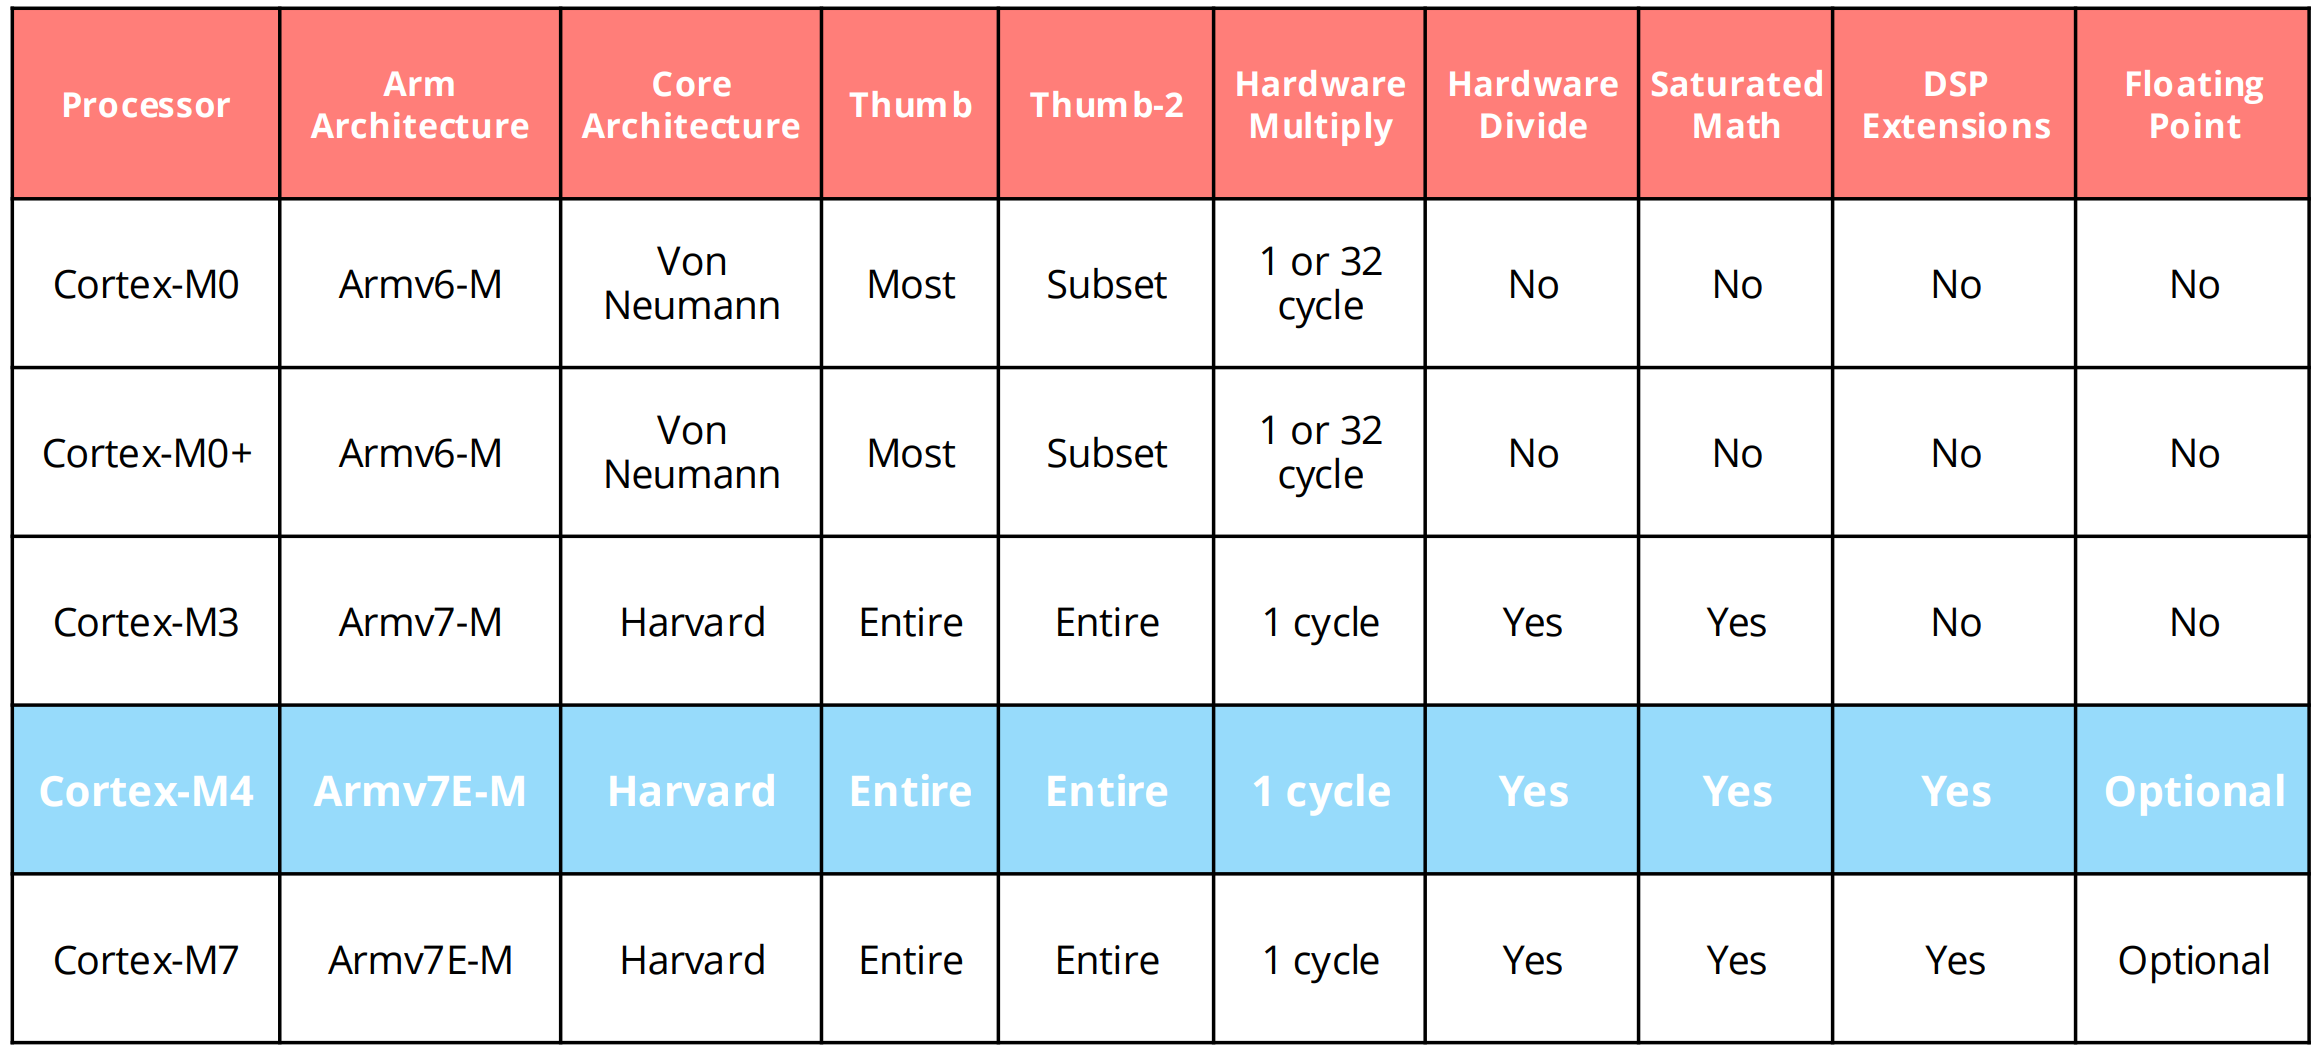
\includegraphics[width=1\linewidth]{img/image10.png}
\end{figure}


\section{Von Neumann Architecture }

The memory holds both data and instructions. CPU \textbf{fetches} instructions from memory, \textbf{decodes} them and
\textbf{executes} them.

The CPU register stores values used internally: program counter (PC), instruction register (IR), generalpurpose registers, etc.

\begin{figure}[H]
    \centering
    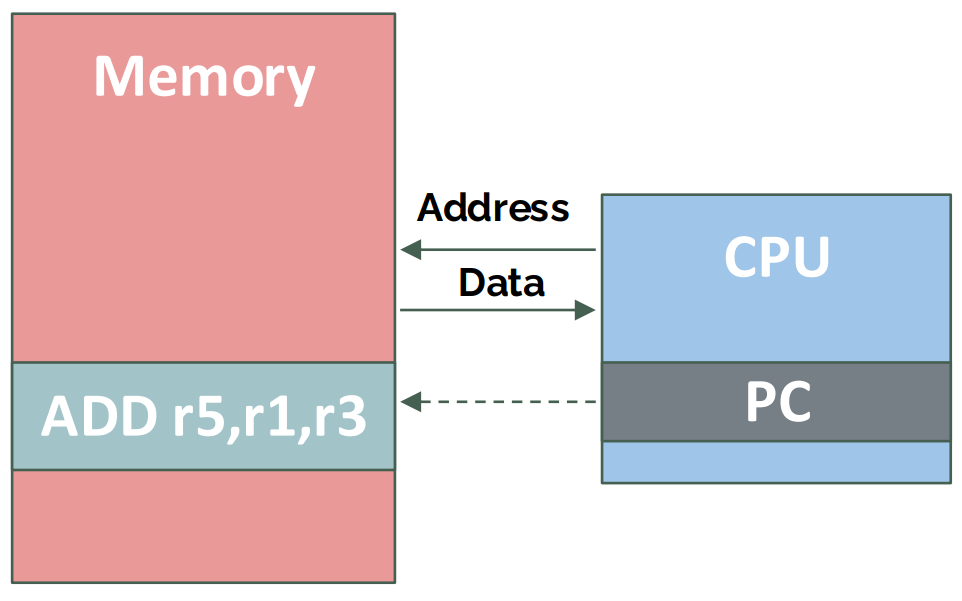
\includegraphics[width=0.4\linewidth]{img/image11.png}
\end{figure}


\section{Harvard Architecture}

There are two separate memories for data and program (instructions). Indeed the processor has two ports
for the two memories, so they don't compete for a single port, this \textbf{allows two simultaneous memory fetches}.

The program counter (PC) always points to program memory (not data memory) which means it cannot use self-modifying
code (secure).

\paragraph{}
Most DSPs are Harvard architectures. The separation of program and data memories provides \textbf{higher
performance}.


\begin{figure}[H]
    \centering
    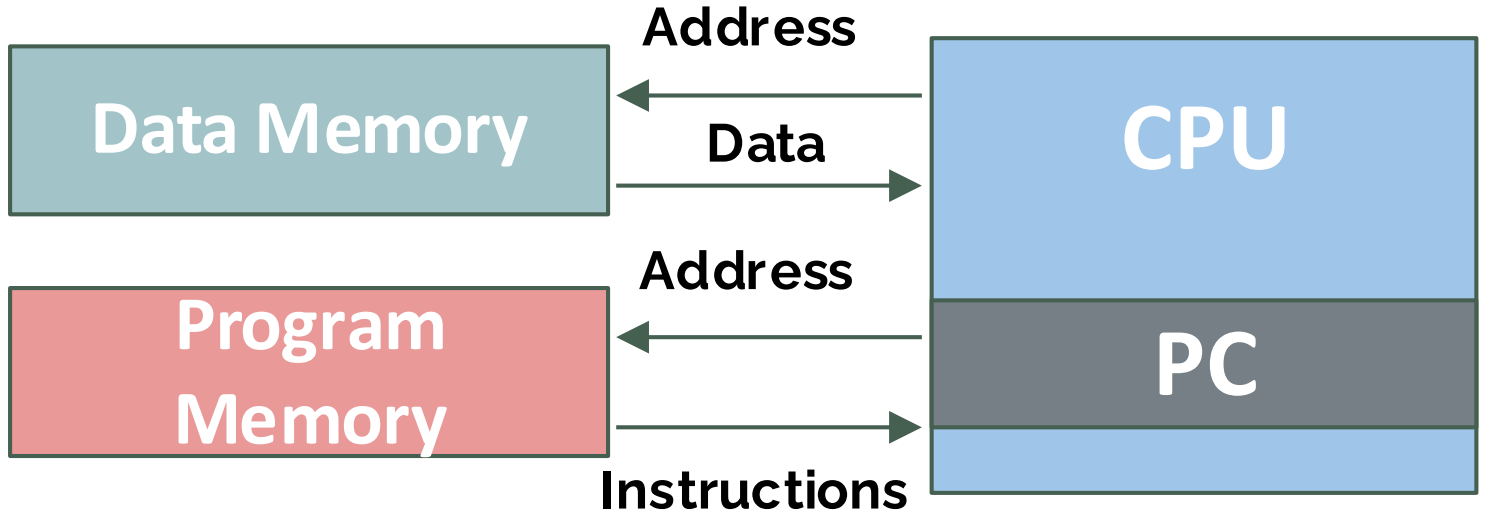
\includegraphics[width=0.5\linewidth]{img/image12.png}
\end{figure}

\section{Cortex-M4 Processor Overview}

The Cortex-M4 processor is designed with a large variety of highly efficient signal processing features
(example: single-cycle multiply accumulate instructions).

\paragraph{}
The \textbf{Multiply-Accumulate} (MAC) Instruction is an important and expensive operation mainly employed in
digital signal processing and video/graphics applications, machine learning included, that computes the
product of two numbers and adds that product to an accumulator.

\paragraph{}
It also features low power consumption, which means a longer battery life on the device that uses it, a
critical non-functional requirement in mobile products.

Furthermore it offers enhanced determinism: critical tasks and interrupt routines can be served quickly in
a known number of cycles. This is crucial for embedded system applications.

\subsection{Cortex-M4 Processor Features}

\textbf{32-bit} reduced instruction set computing (RISC) processor, \textbf{Harvard architecture}, so separate data bus and instruction bus and it has 3-stage + \textbf{branch speculation pipeline}.

\paragraph{}
It supports sleep modes: Features wake-up interrupts, with wait for interrupt (WFI) and wait for event (WFE) instructions.

Enhanced instructions Hardware divid, MAC, and so on.

\begin{figure}[H]
    \centering
    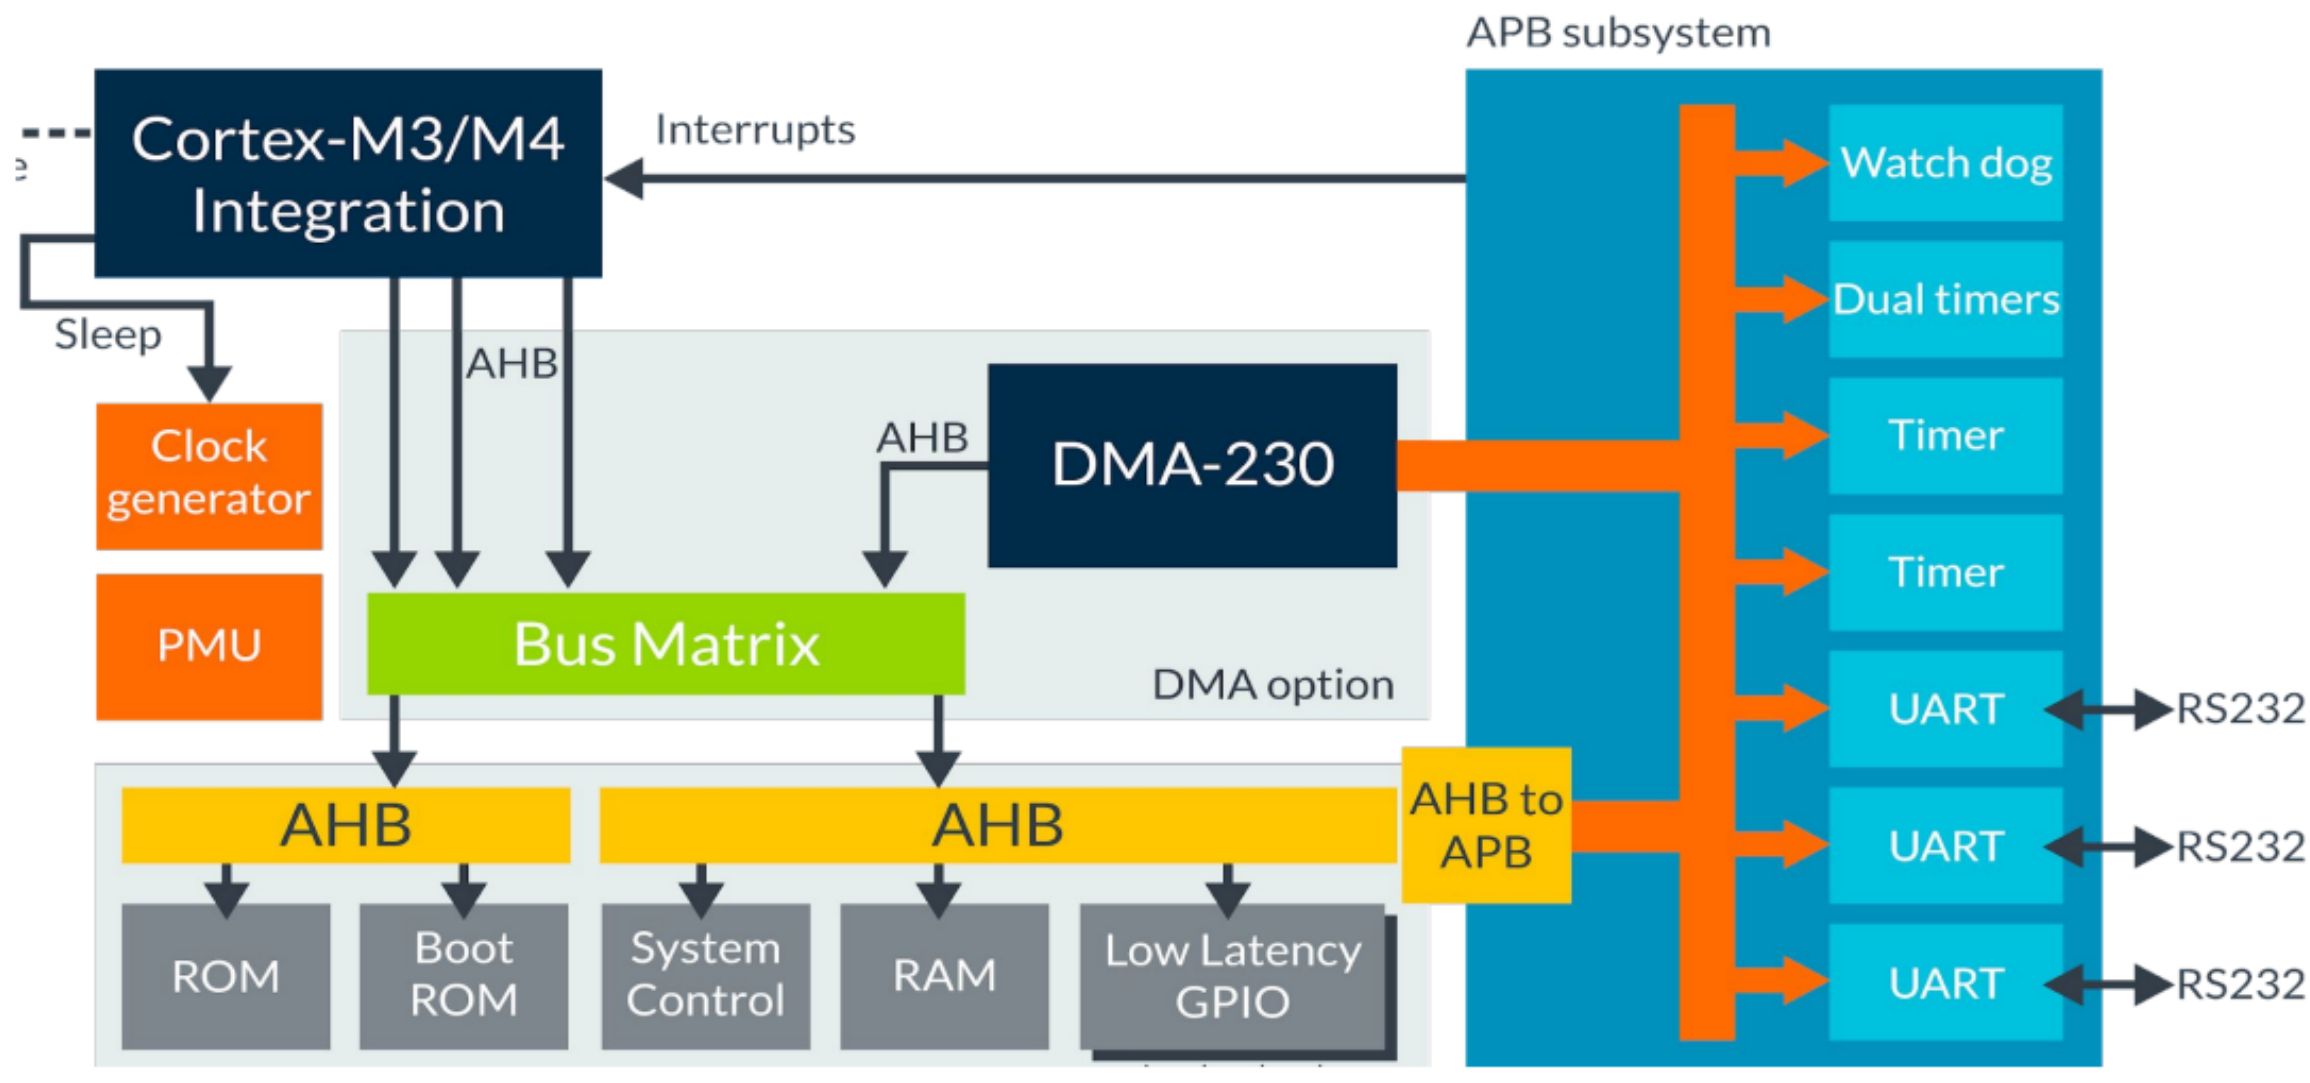
\includegraphics[width=1\linewidth]{img/image13.png}
    \caption{Arm M4-MCU Architecture}
\end{figure}

\subsection{Cortex-M4 Block Diagram}

\begin{figure}[H]
    \centering
    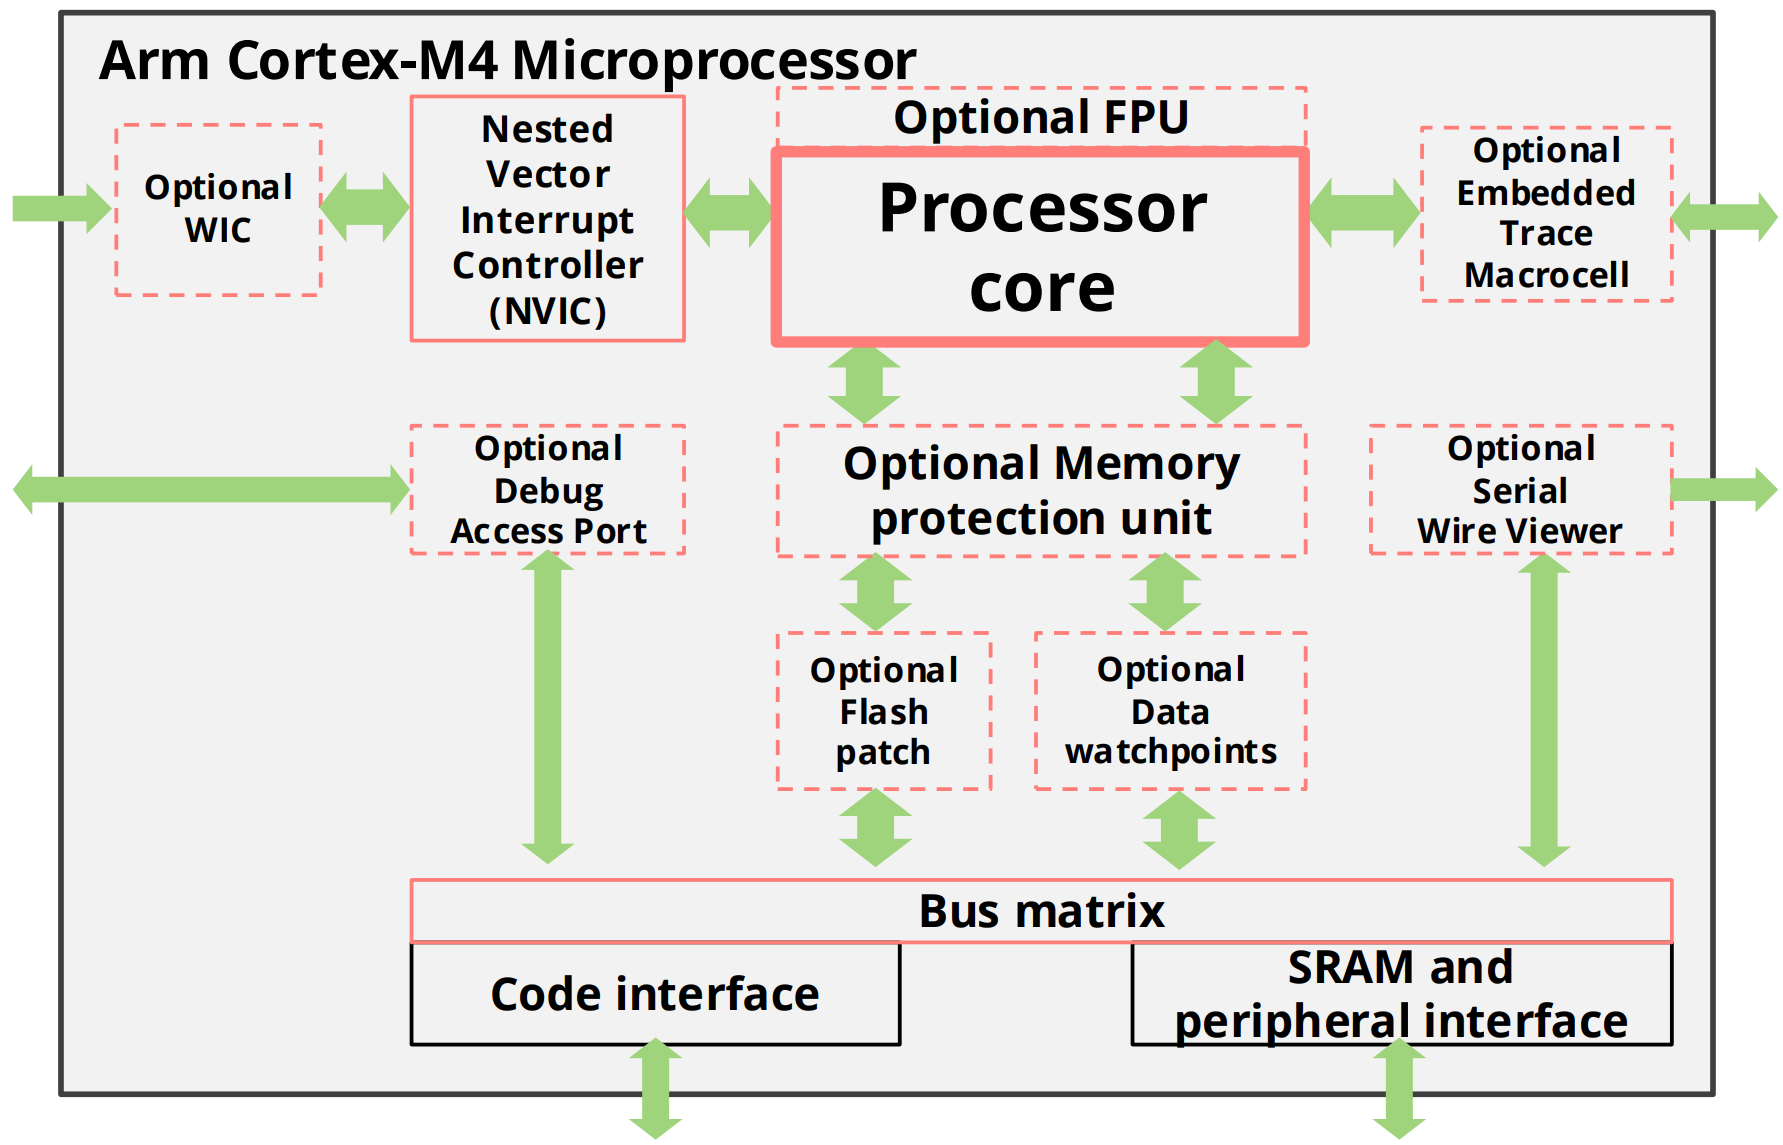
\includegraphics[width=0.8\linewidth]{img/image14.png}
\end{figure}

Here are the components as described:

\subsubsection{Processor core}

The processor core contains internal registers, the ALU, data path and some control logic.

It has a three-stage pipeline: fetch, decode, execution. Some instructions may take multiple cycles to
execute in which case the pipeline will be stalled. Also the pipeline speculatively prefetches instructions
from branch target addresses.

\begin{figure}[H]
    \centering
    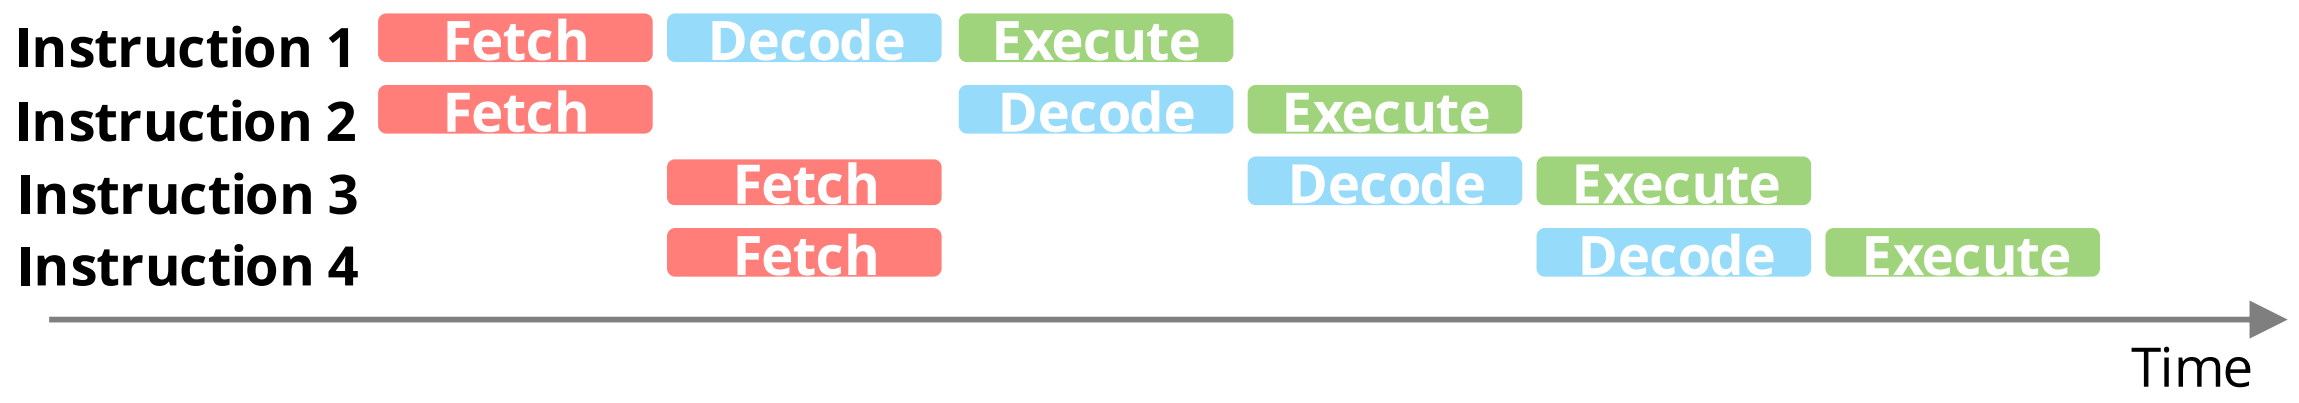
\includegraphics[width=0.8\linewidth]{img/image15.png}
\end{figure}

\subsubsection{Nested vectored interrupt controller (NVIC)}
It automatically handles nested interrupts, such as comparing priorities between interrupt requests and
the current priority level.

\subsubsection{Wake-up interrupt controller (WIC)}
For low-power applications, the microcontroller can enter sleep mode by shutting down most of the
components.

When an interrupt request is detected, the WIC can inform the power management unit to power up the
system.

\subsubsection{Memory protection unit (MPU)}

It is used to protect memory content. It makes some memory regions read-only and prevents user
applications from accessing each other.


\subsubsection{Debug subsystem - Embedded Trace Macrocell and Serial Wire Viewer}

It handles debug control, program breakpoints, and data watchpoints.


When a debug event occurs it can put the processor core in a halted state, so that developers can
analyse the status of the processor like register values and flags at that point.

\subsubsection{Bus matrix/Bus interconnect}

It provides data transfer management among hardware components and peripherals.

It also allows data transfer to take place on different buses simultaneously:

\begin{itemize}
    \item Advanced High-performance Bus (AHB)-Lite bus for high bandwidth peripherals
    \item Advanced Peripheral Bus (APB) interface. Low-power, meant for peripherals such as timers, interrupt controllers, UARTs, I/O
\end{itemize}

The bus matrix may include bus bridges (example: AHB-to-APB bus bridge) to connect different buses
into a network using a single global memory space.


\section{Programming Model}

The programming/programmer model is the set of registers available for use by programs.

The CPU has many other special purpose registers that are used for internal operations, which are
unavailable to programmers.


\subsection{Arm Cortex-M4 Processor Registers}

\begin{figure}[H]
    \centering
    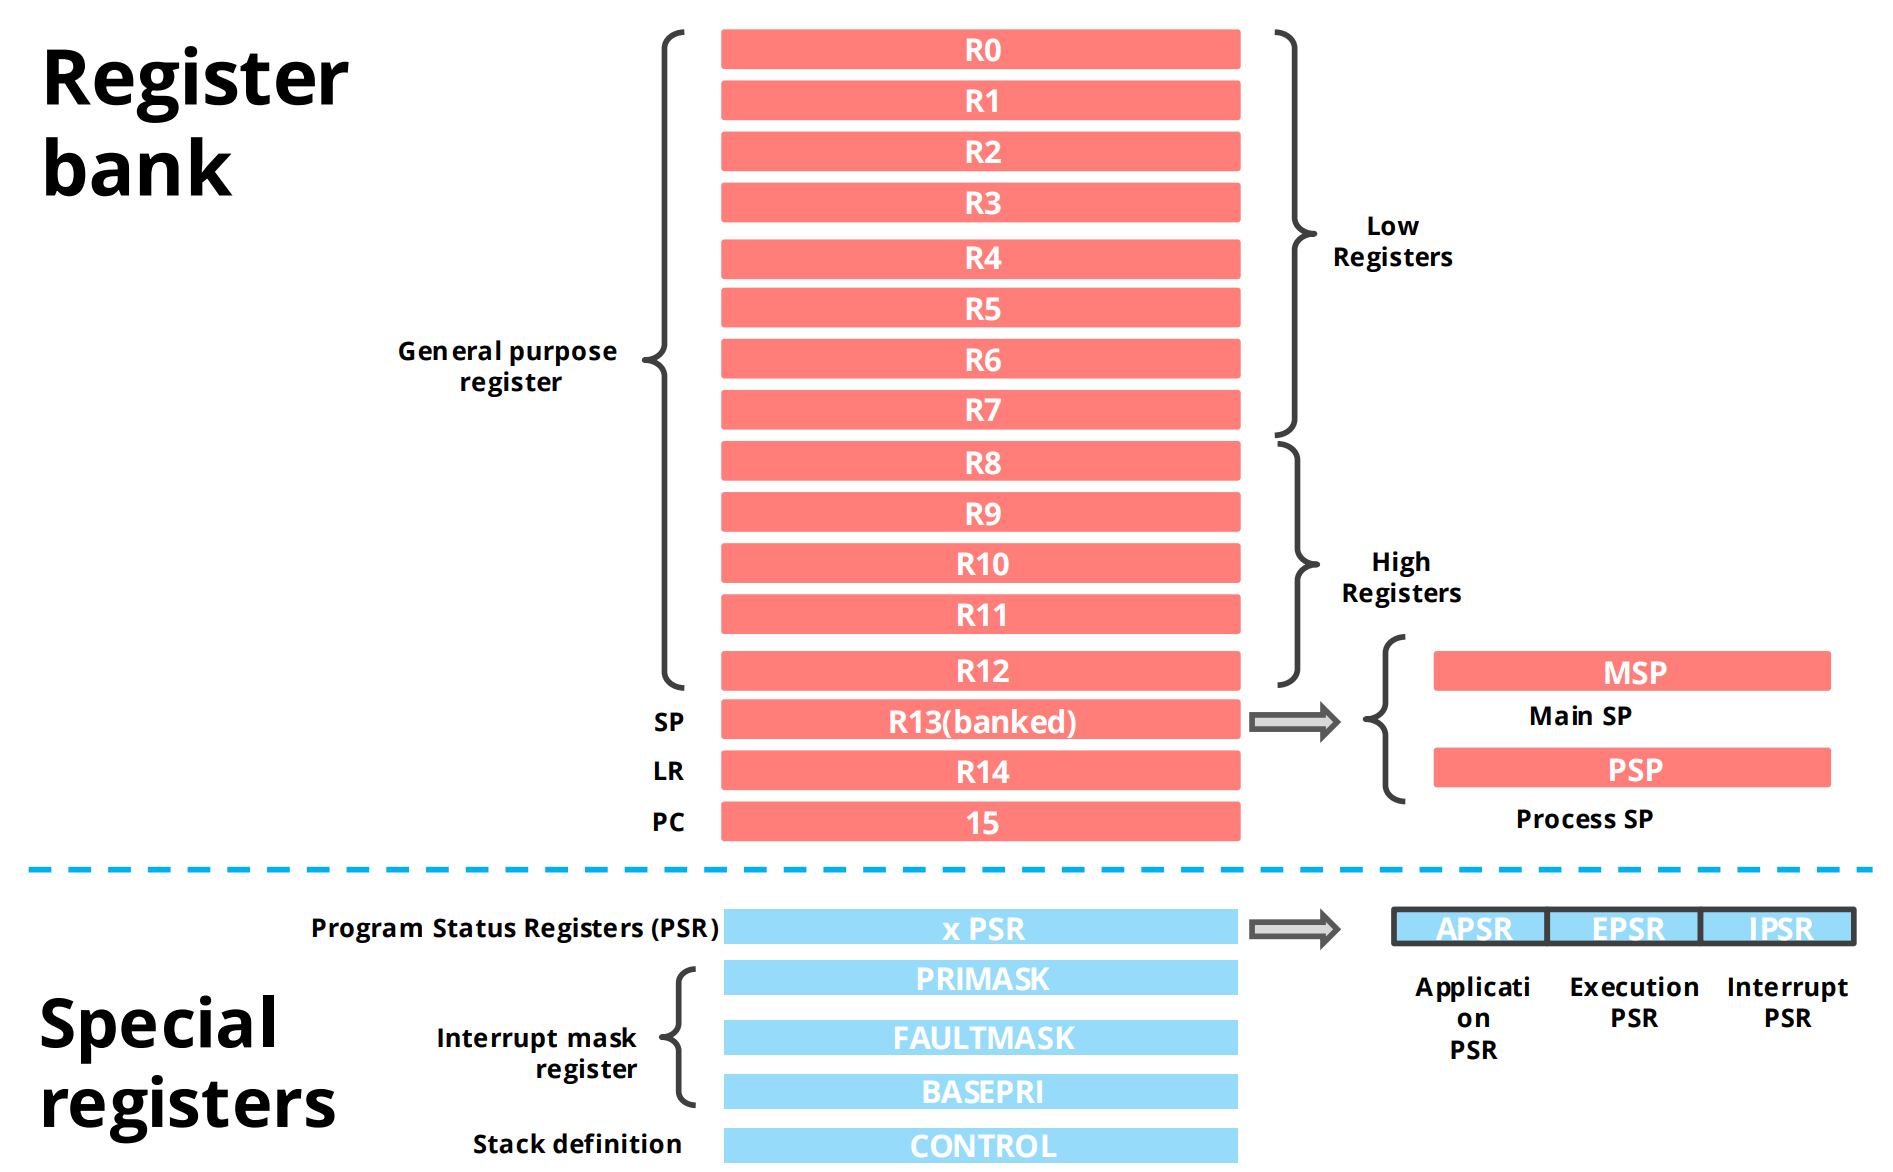
\includegraphics[width=0.8\linewidth]{img/image16.png}
\end{figure}


The processor registers store and process temporary data within the processor core quickly.


They follow a load-store architecture, in which to process memory data, they first have to be loaded from
memory to registers, processed inside the processor core using register data only, and then written back
to memory if needed.

\paragraph{}
The Cortex-M4's register bank is composed of 16 X 32-bit registers (R0-R12 are general-purpose, others
are the stack pointer (R13), the link register (R14) and the program counter (R15)).

\subsubsection{Stack Pointer}
The stack pointer (SP) records the current address of the stack and is used for saving context while
switching between tasks.

The Cortex-M4 has two SPs: the main SP, used in applications that require privileged access like the OS
kernel, and the process SP which is used in base-level application code.


\subsubsection{Program Counter}

The program counter (PC) records the address of the current instruction code and is automatically
incremented.

\begin{figure}[H]
    \centering
    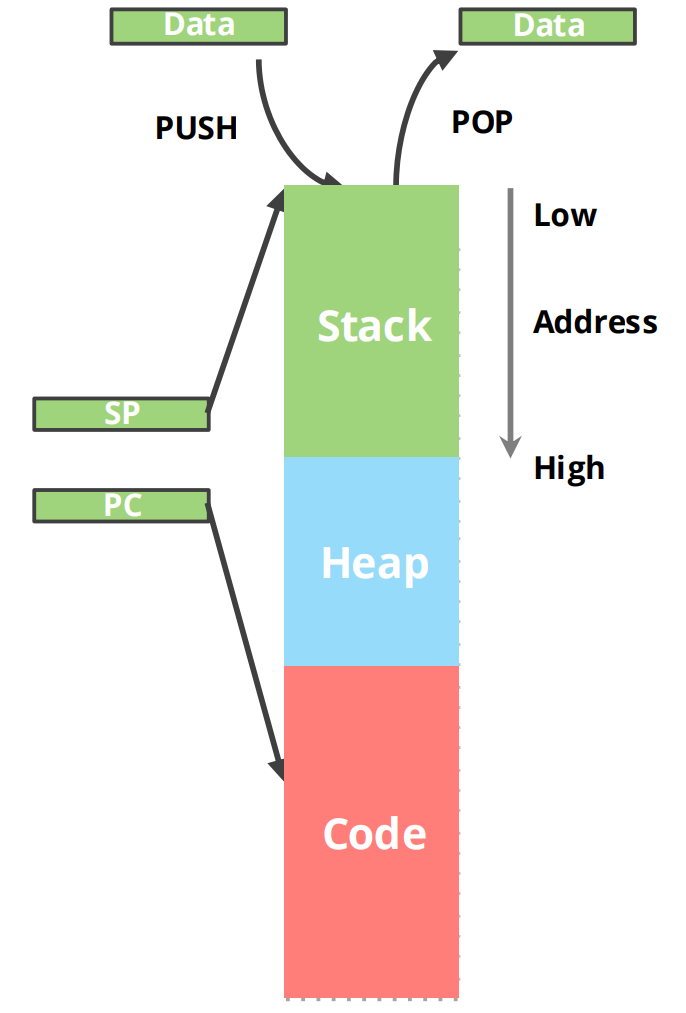
\includegraphics[width=0.25\linewidth]{img/image17.png}
\end{figure}

\subsubsection{Linik Register}
The link register (LR) stores the return address of a subroutine or function call. The PC will load the
value from the LR after a function is finished.

\begin{figure}[H]
    \centering
    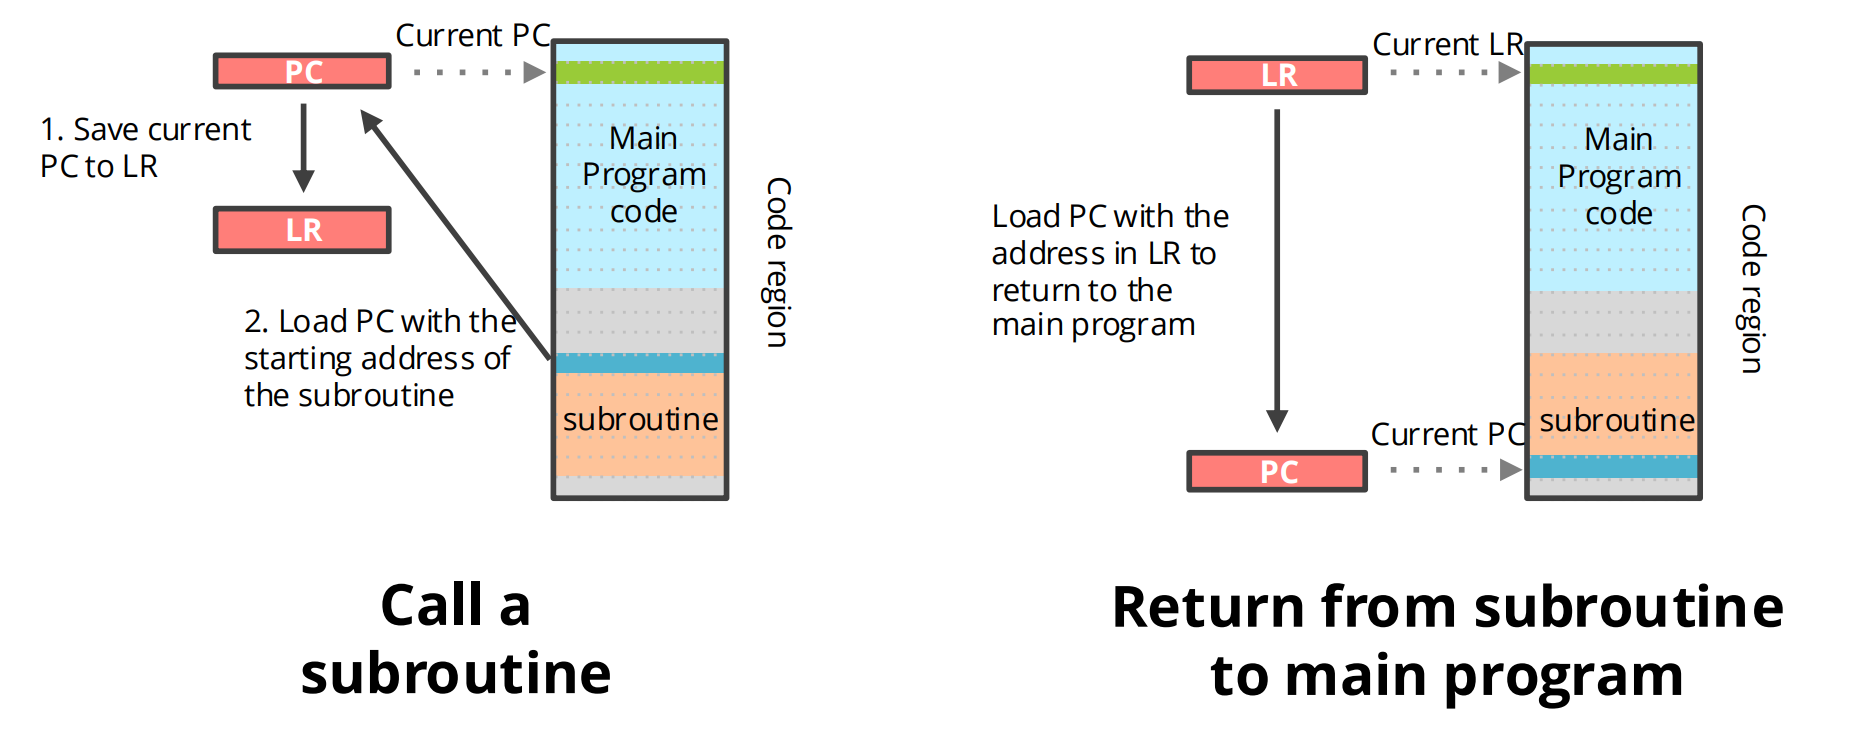
\includegraphics[width=0.85\linewidth]{img/image18.png}
\end{figure}

\subsection{Cortex-M4 Registers (Special Registers)}
Then there are special registers like the interrupt mask register used to enable/disable interrupts, the
program status registers (PSR) to understand what kind of exceptions, interruptions and results occurred.

\paragraph{}
The \textbf{xPSR}, \textbf{combined program status register}, provides information about program execution and
Arithmetic Logic Unit (ALU) flags. It combines the Application PSR, Interrupt PSR and Execution PSR.

\begin{figure}[H]
    \centering
    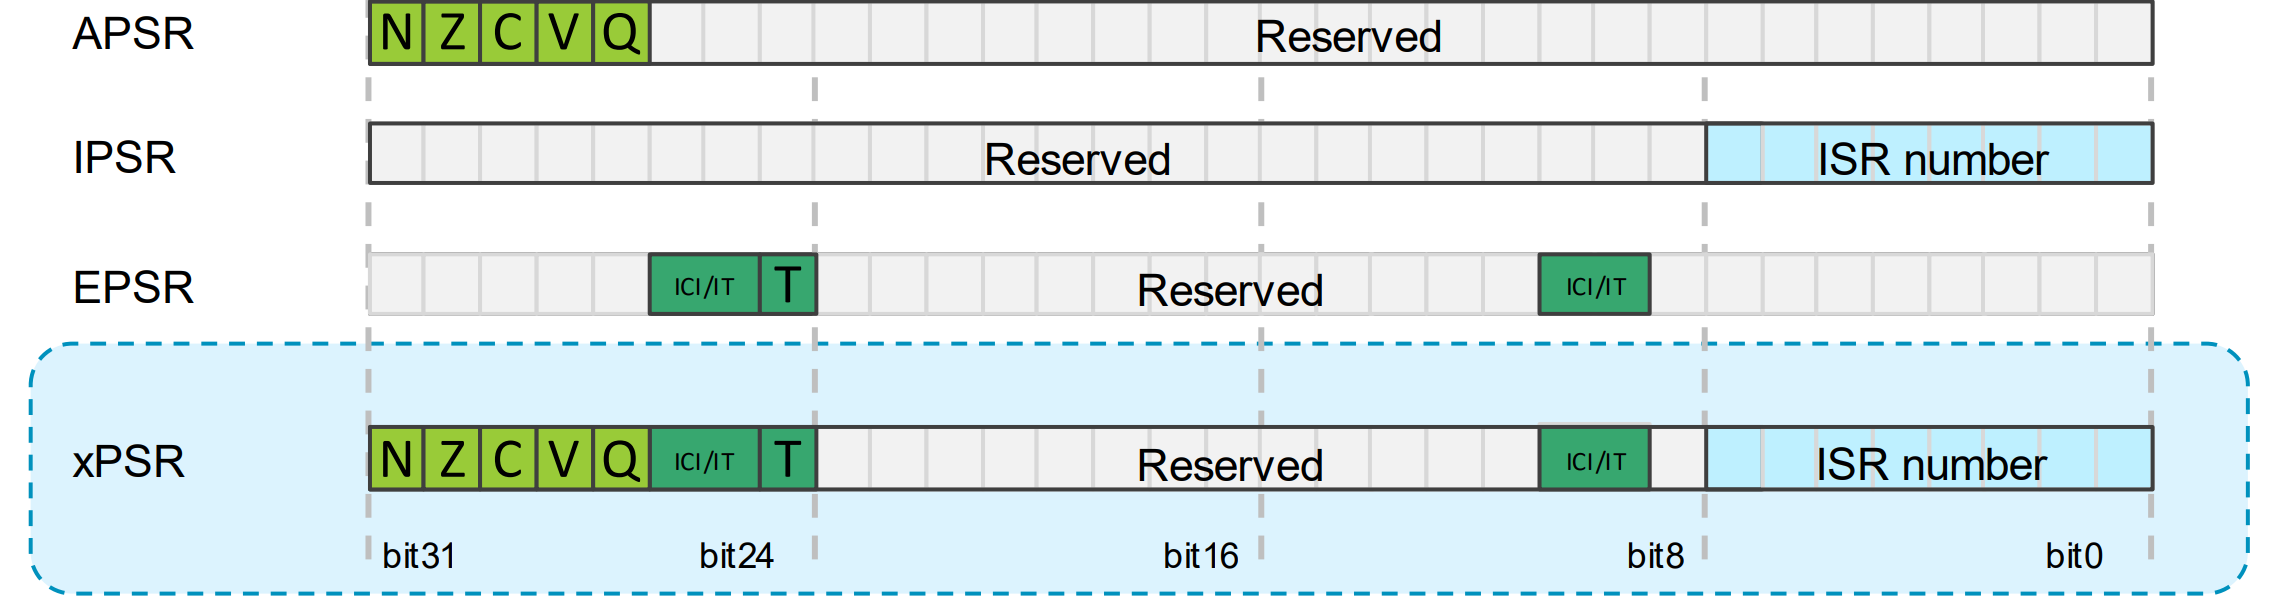
\includegraphics[width=1\linewidth]{img/image19.png}
\end{figure}

\paragraph{APSR - Application Program Status Register}

\begin{itemize}
    \item[-] N: negative flag
    \item[-] Z: zero flag
    \item[-] C: carry flag
    \item[-] V: overflow flag
    \item[-] Q: stick saturation flag
\end{itemize}


\section{Arm Cortex-M4 Memory Map}

The \textbf{memory map} describes the organization of the \textbf{processor’s address space}.

ARM memory is \textbf{byte-addressable} using \textbf{32-bit} addresses. The Cortex-M4 processor has \textbf{4GB of memory address space}.

The 4GB memory address space is architecturally defined with a number of regions, each one designed
for particular recommended use cases, making it easy for a software programmer to port between
different devices.

\paragraph{}
Memory map can also be flexibly defined by the user, apart from some fixed memory addresses such as
internal private peripheral bus.


\begin{figure}[H]
    \centering
    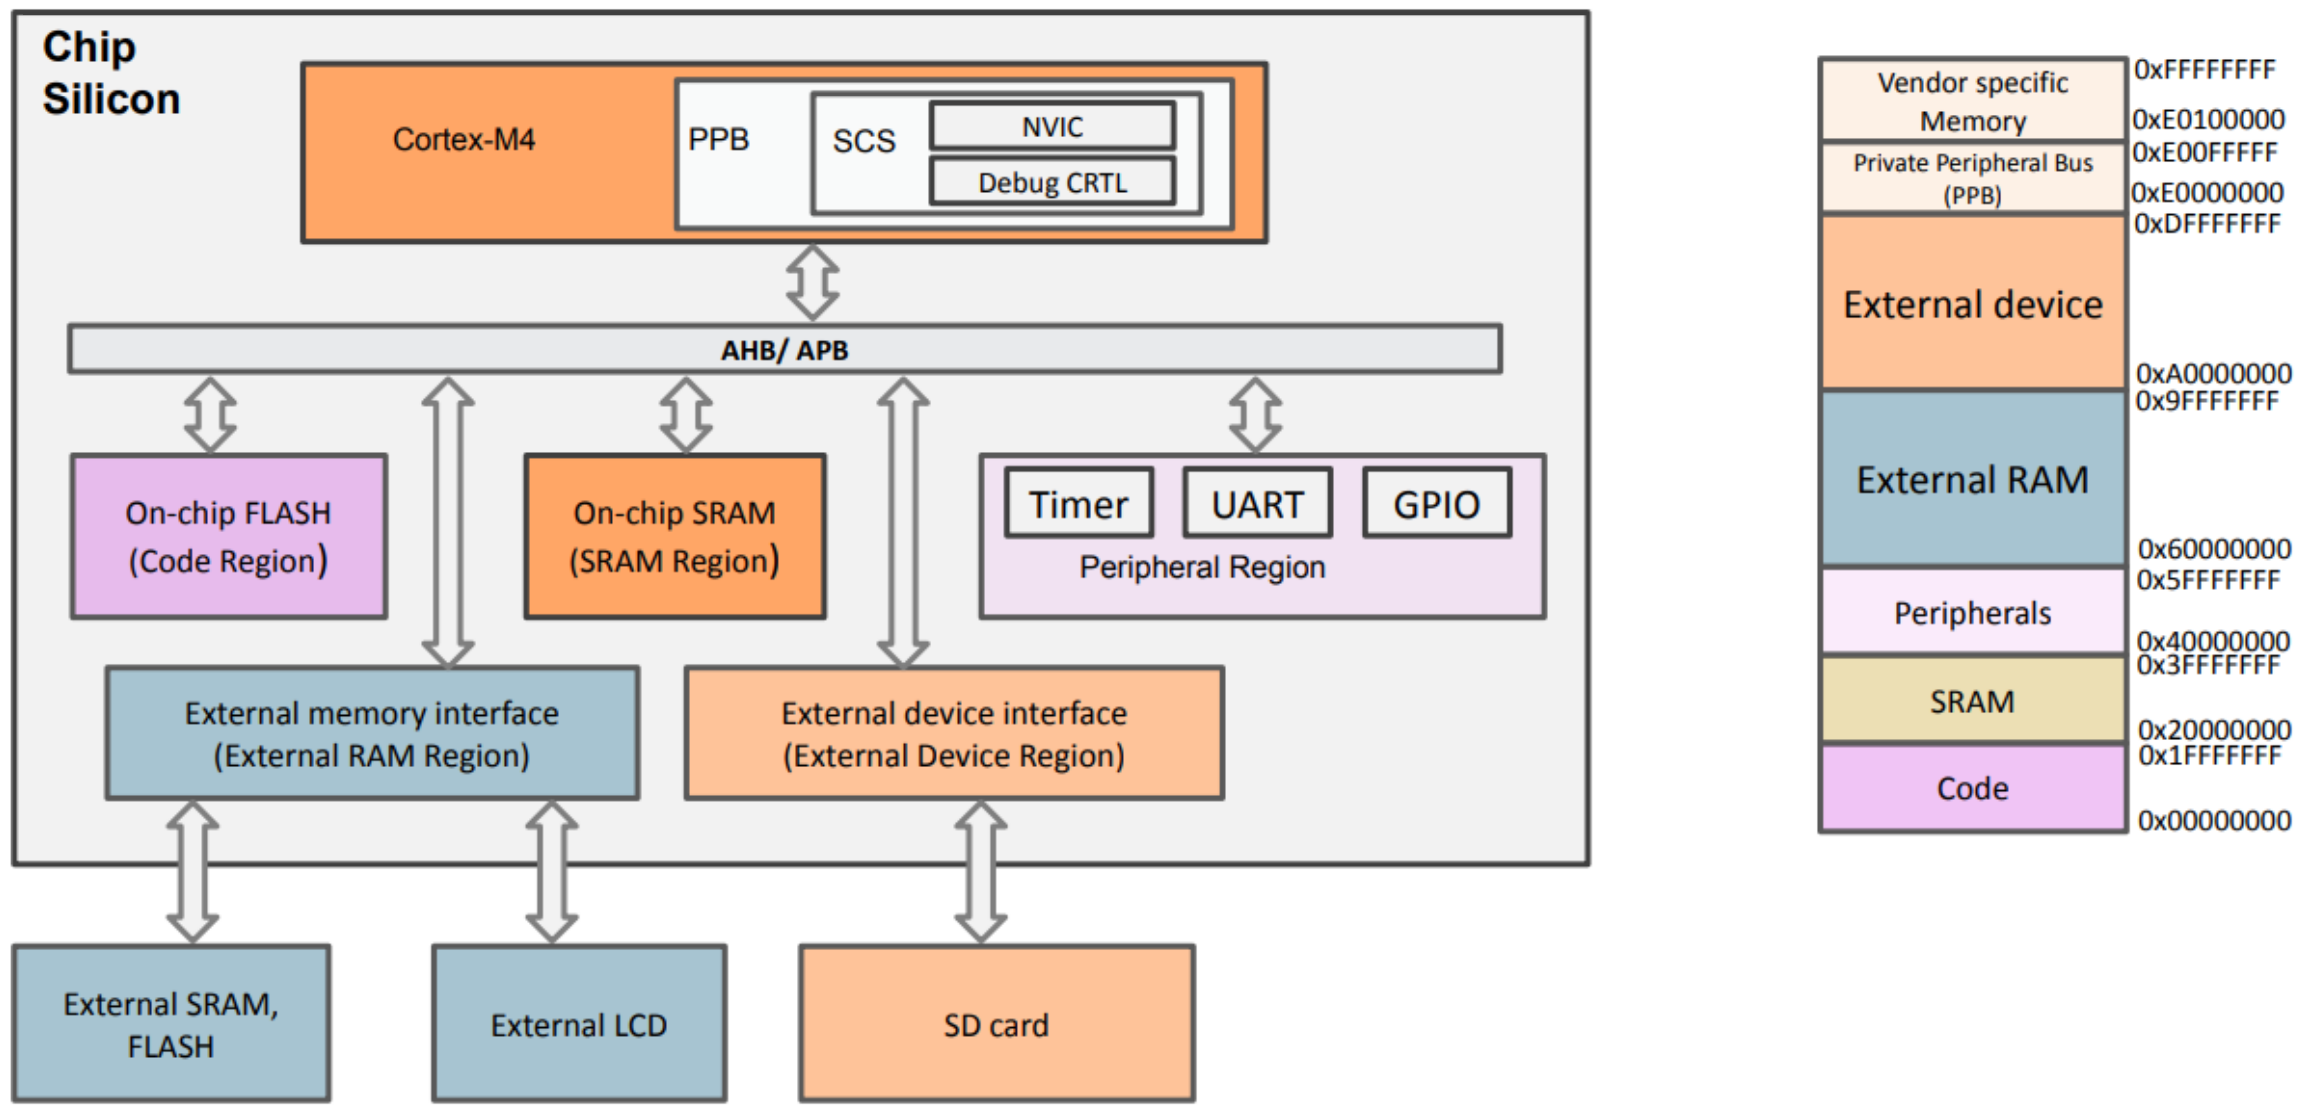
\includegraphics[width=1\linewidth]{img/image20.png}
\end{figure}


\begin{figure}[H]
    \centering
    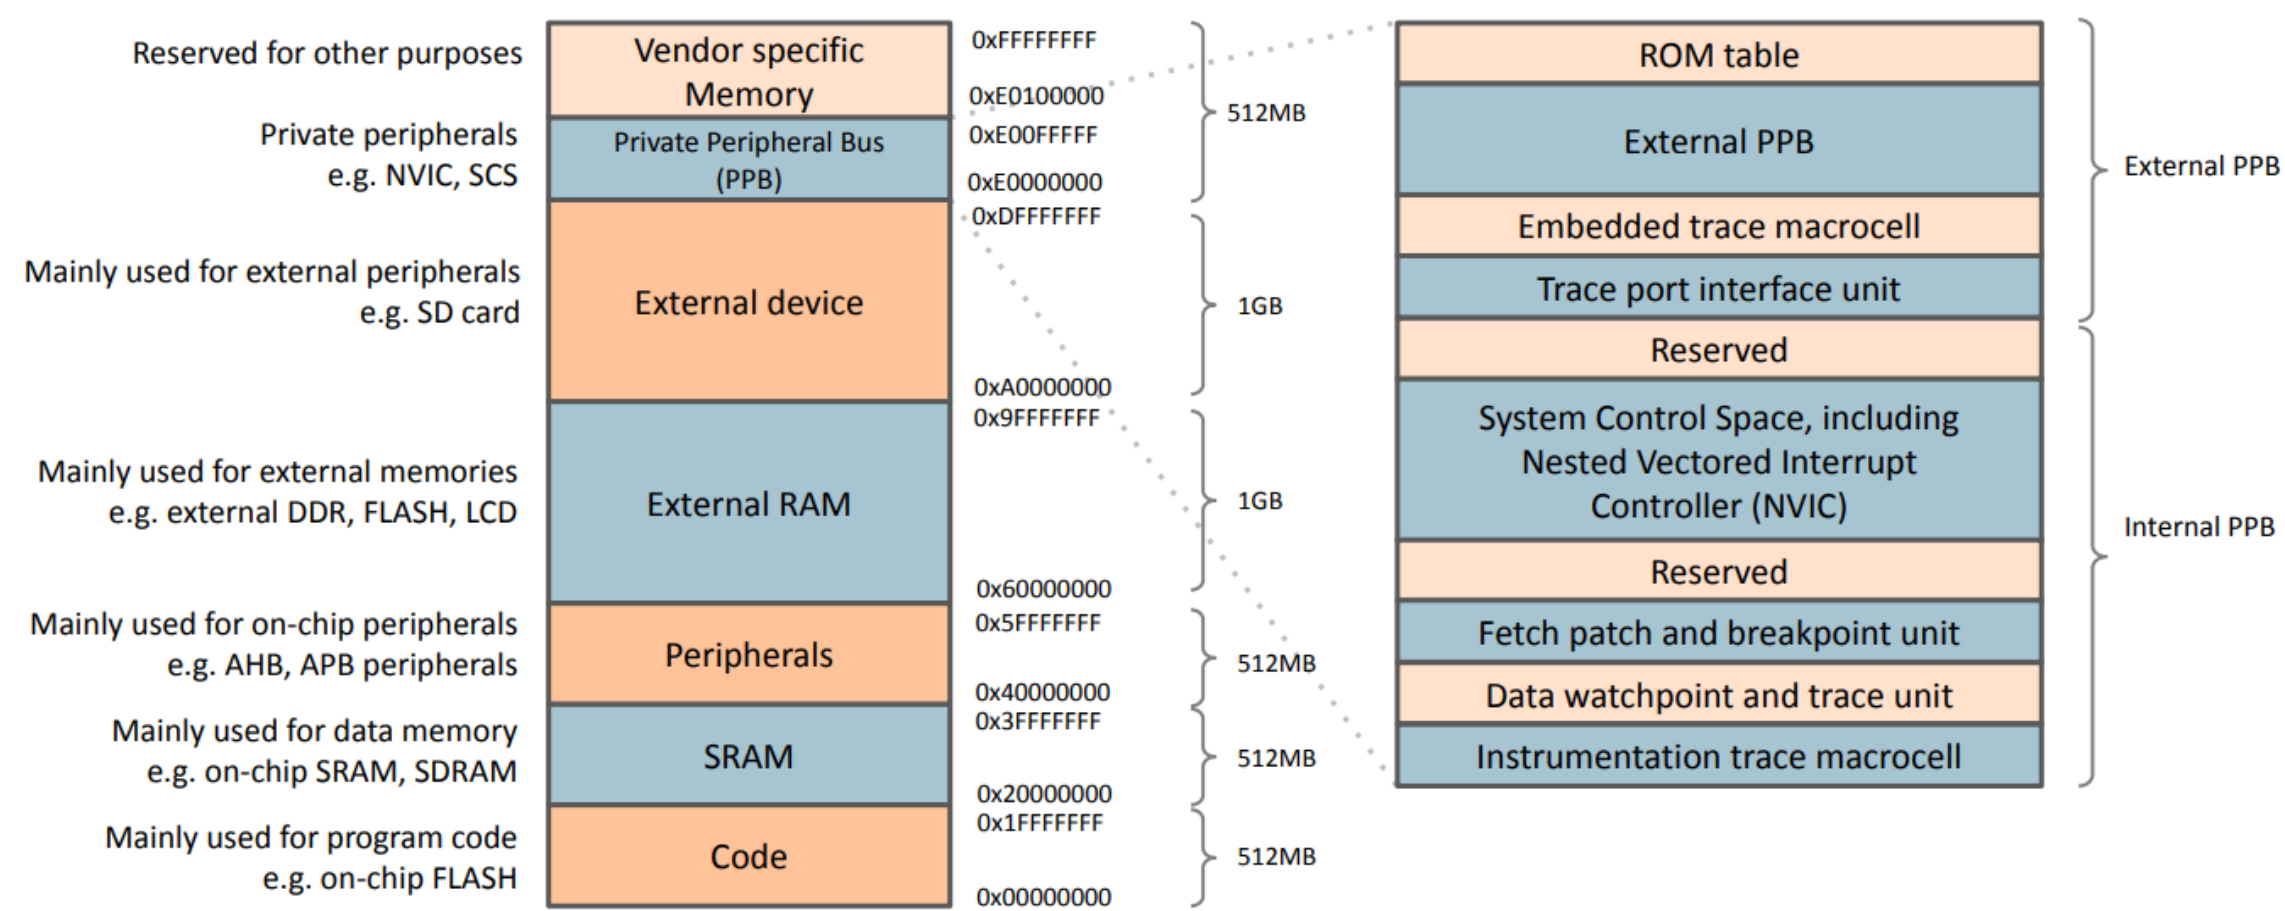
\includegraphics[width=1\linewidth]{img/image21.png}
\end{figure}


\paragraph{Code Region} It is primarily used to store program code, can also be used for data memory.
On-chip memory, such as on-chip FLASH.

\paragraph{SRAM Region} It is primarily used to store data, such as heaps and stacks. It can also be used to store program code.

\paragraph{Peripheral Region} It is primarily used for AHB/APB peripherals.
\paragraph{External RAM region} It is primarily used to store large data blocks or memory caches. It's an off-chip memory, slower than onchip SRAM region.
\paragraph{External device region} Used to map external, off-chip devices like SD cards.
\paragraph{Private Peripheral Bus (PPB)} Provides access to internal and external processor resources.


\section{Bit-band Operations}
One interesting property of Arm architectures is that they allow bit-band operations.

Bit-band operations allow a single load/store operation to access a single bit in the memory, without
having to access 32 bits at once just to change a single one.

It works by directly writing a single bit (0 or 1) to the "\textbf{bit-band alias address}" of the data.


\paragraph{Bit-band Alias Address}

SRAM and Peripheral regions include \textbf{bit band} and \textbf{bit band alias} areas.

\begin{figure}[H]
    \centering
    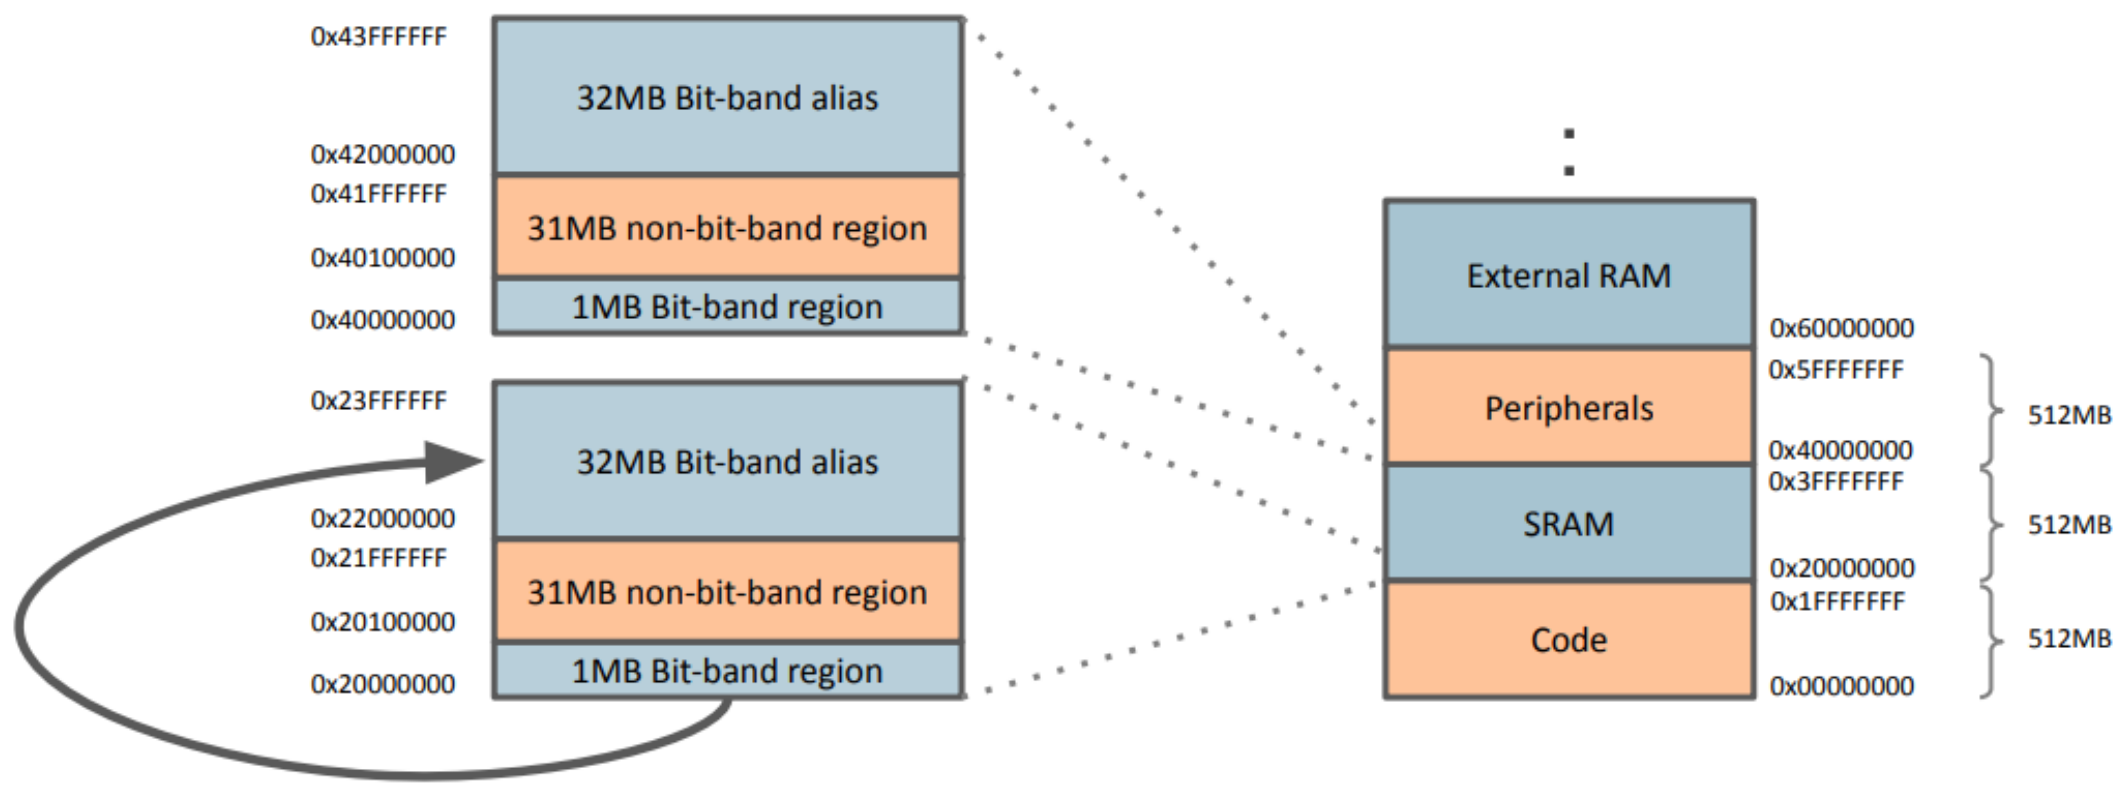
\includegraphics[width=1\linewidth]{img/image22.png}
\end{figure}

Each bit of the data is one-to-one mapped to the bit-band alias address. Each bit has an address multiple
of 4.


1 byte = 8 bits = 4x8 = 32 addresses in memory space.


\subsection{Benefits of bit-band operations}

Bit-band operations allow for \textbf{faster bit operations} and \textbf{fewer instructions}. It's an \textbf{atomic operation}, so it helps prevent data conflict hazards.

\newpage
\section{Cortex-M4 Endianness}

Endian refers to the order of bytes stored in memory.

\paragraph{Little endian:} lowest byte of a word-size data is stored in bit 0 to bit 7
\paragraph{Big endian: } lowest byte of a word-size data is stored in bit 24 to bit 31


Cortex-M4 supports both little endian and big endian. However, endianness only exists in the hardware level.


\begin{figure}[H]
    \centering
    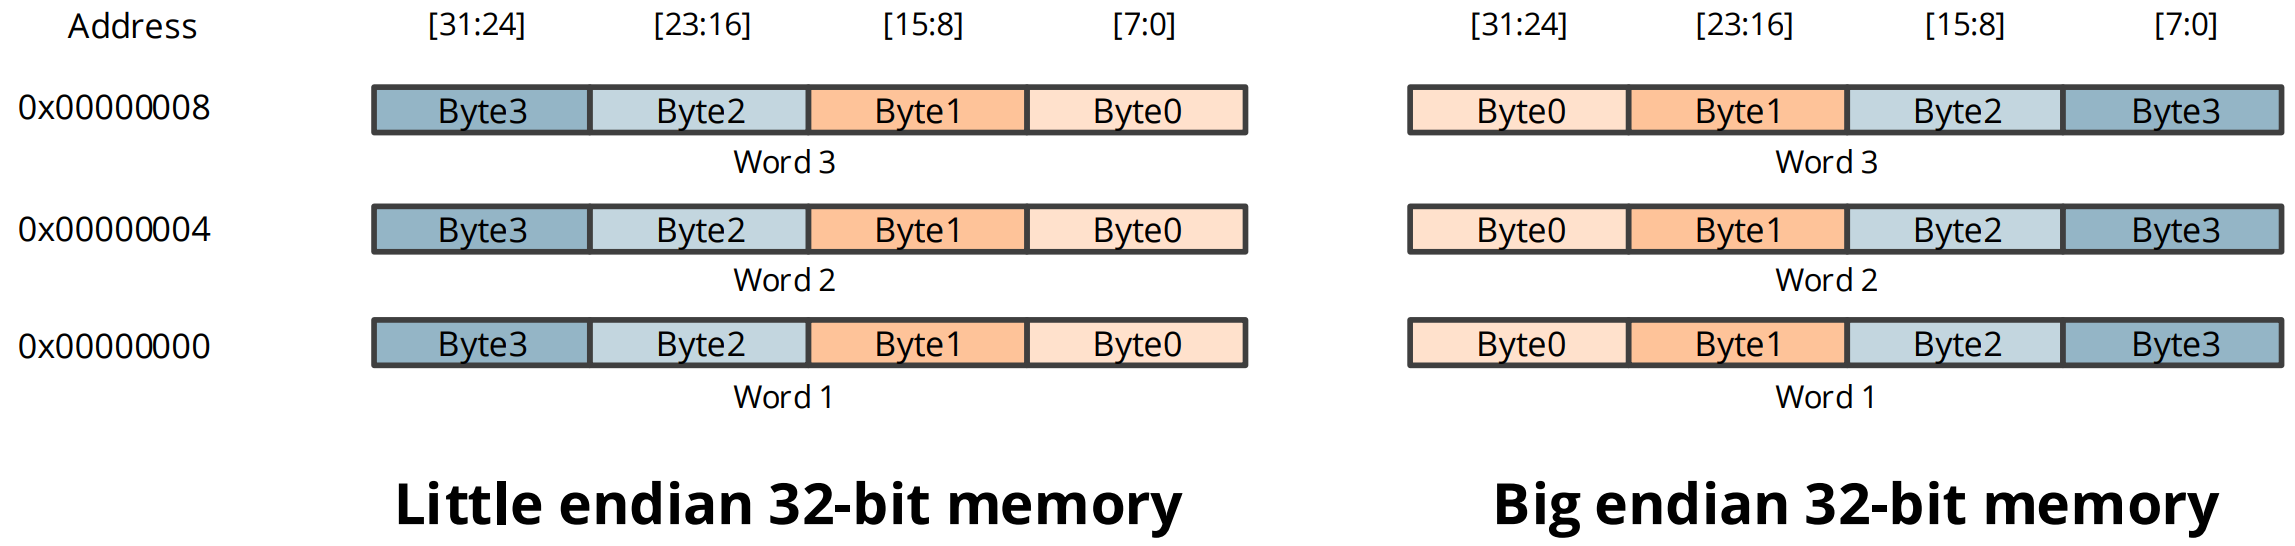
\includegraphics[width=1\linewidth]{img/image23.png}
\end{figure}


\section{Arm and Thumb Instruction Set}

The early Arm instruction set was a 32-bit instruction set called the Arm instructions. It's powerful and
performs well but it required a larger program memory and a larger power consumption.

\paragraph{Example: } ADDS Rd, Rd, \#Constant


\begin{figure}[H]
    \centering
    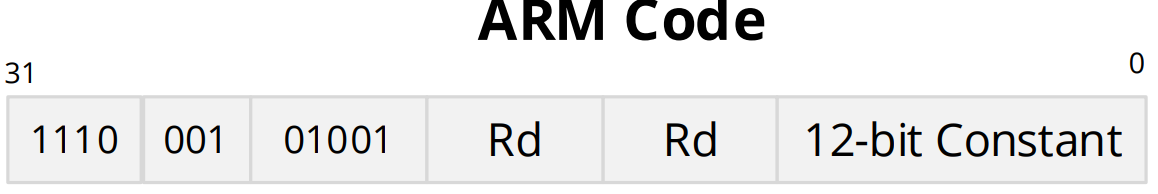
\includegraphics[width=0.7\linewidth]{img/image25.png}
\end{figure}

\paragraph{Thumb Code} ADD Rd, \#Constant


\begin{figure}[H]
    \centering
    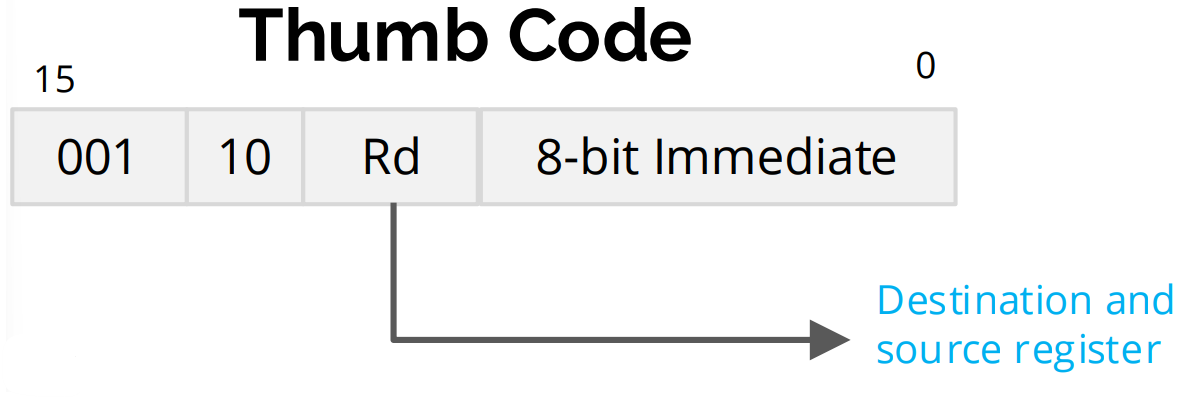
\includegraphics[width=0.6\linewidth]{img/image26.png}
\end{figure}

The instruction does the same operation but encoded using \textbf{less number of bits}!

\paragraph{}

Later on Arm introduced the Thumb-1 instruction set. It had 16-bit instructions as it was a subset of the
Arm instruction set.

\paragraph{}
Code size is reduced by -30\% but performance is also reduced by -20\%.

A multiplexer is used to switch between the two sets, which requires a switching overhead. This is so one
can benefit from 32-bit Arm's high performance and 16-bit Thumb-1's high code density (reduced program code size, Sometimes leads to an increased number of instructions, thus making thumb
slower to execute because fetching instructions is slower than executing instructions).

The processor
and the compiler manage this automatically.


\begin{figure}[H]
    \centering
    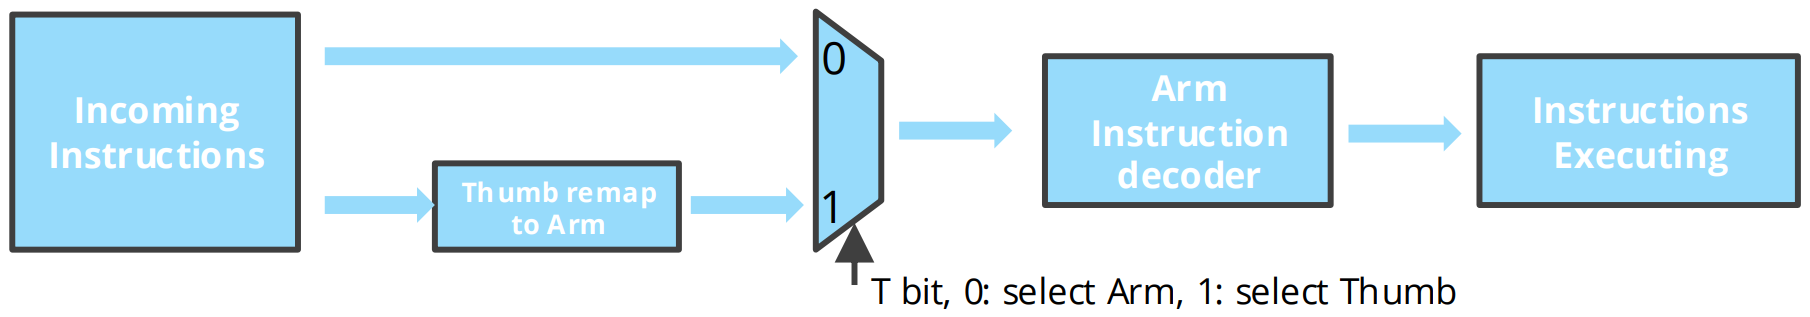
\includegraphics[width=0.8\linewidth]{img/image27.png}
\end{figure}

\paragraph{The Thumb-2} instruction set consists of both 32-bit Thumb instructions and the original 16-bit Thumb-1
instruction sets. Compared to the 32-bit Arm instruction set, code size is reduced by -26\% with similar
performance.

The Thumb-2 instruction set also covers almost all functionality of the Arm instruction set and most
instructions are \textbf{unconditional}, whereas almost all Arm instructions are conditional.